\documentclass[tikz,border=6pt]{standalone}

\usepackage{amsmath}
\usepackage{amssymb}
\usepackage{fontspec}



\usetikzlibrary{
    arrows.meta,
    decorations.pathmorphing
}

\begin{document}

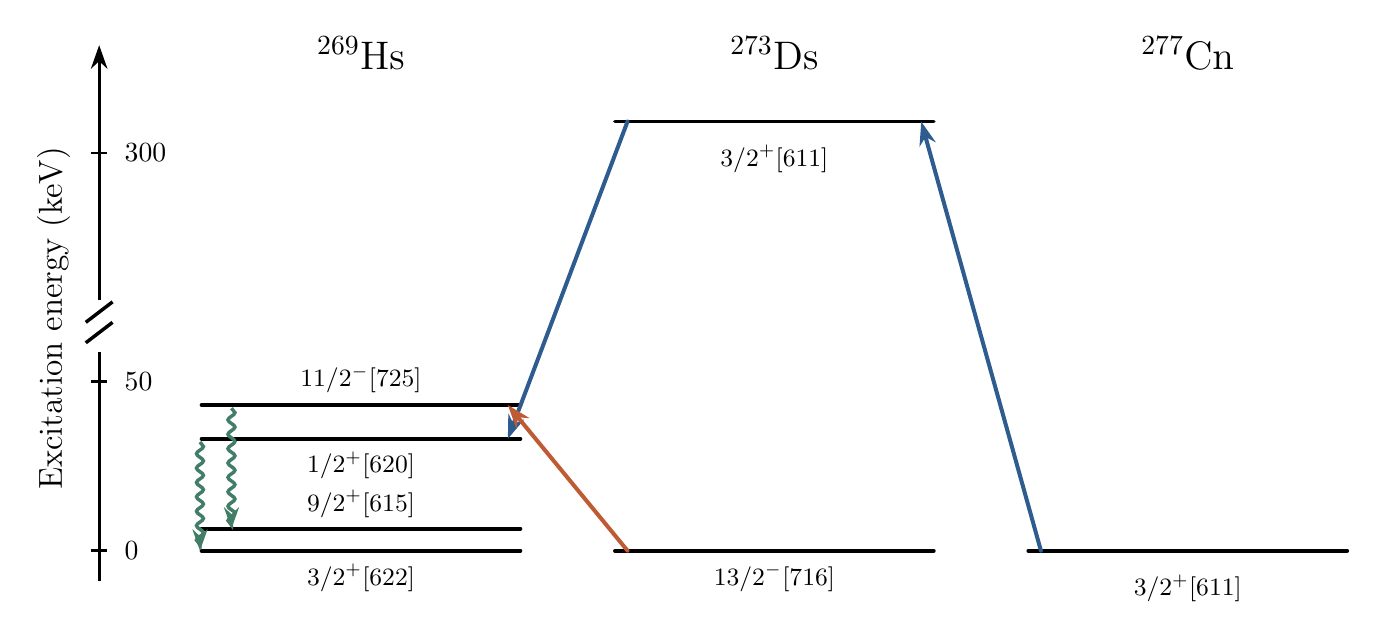
\begin{tikzpicture}[
    x=1cm,
    y=1cm,
    level/.style={
        line width=1.35pt,
        line cap=round
    },
    transition/.style={
        -{Stealth[length=3.0mm,width=2.1mm]},
        line width=1.45pt,
        line cap=round
    },
    gamma/.style={
        decorate,
        decoration={
            snake,
            amplitude=1.25pt,
            segment length=5.2pt
        },
        -{Stealth[length=2.7mm,width=1.9mm]},
        line width=1.25pt
    },
    state/.style={
        font=\small,
        inner sep=1pt
    },
    nucleus/.style={
        font=\Large\bfseries
    },
    ticklabel/.style={
        font=\normalsize
    }
]

% ============================================================
% Muted scientific colors
% ============================================================

\definecolor{branchblue}{RGB}{47,92,143}
\definecolor{branchorange}{RGB}{190,91,52}
\definecolor{gammagreen}{RGB}{66,125,103}

% ============================================================
% Common vertical coordinates
% ============================================================

% Ground-state reference
\def\yZero{1.20}

% 269Hs excited states
\def\yHsFive{1.48}       % 5.8 keV
\def\yHsThirty{2.62}     % 30 keV
\def\yHsForty{3.05}      % approximately 40 keV

% Axis reference ticks
\def\yFifty{3.35}        % 50 keV
\def\yThreeHundred{6.25} % 300 keV

% Broken-axis positions
\def\yBreakLow{3.72}
\def\yBreakHigh{4.38}

% 273Ds first excited state
\def\yDsExcited{6.65}    % approximately 320 keV

% ============================================================
% Horizontal coordinates
% ============================================================

% Right-to-left chain: 277Cn -> 273Ds -> 269Hs.
\def\xAxis{0.00}
\def\xRHsL{1.30}
\def\xRHsR{5.35}
\def\xRDsL{6.55}
\def\xRDsR{10.60}
\def\xCnL{11.80}
\def\xCnR{15.85}
% 277Cn ground-state reference.
\def\yCnState{\yZero}

% ============================================================
% Central excitation-energy axis
% ============================================================

% Lower continuous section
\draw[line width=1.05pt]
    (\xAxis,0.82)
    --
    (\xAxis,\yBreakLow);

% Upper continuous section
\draw[line width=1.05pt]
    (\xAxis,\yBreakHigh)
    --
    (\xAxis,7.25);

% Arrow at the top of the axis
\draw[
    -{Stealth[length=3.0mm,width=2.1mm]},
    line width=1.05pt
]
    (\xAxis,7.25)
    --
    (\xAxis,7.62);

% ------------------------------------------------------------
% Axis ticks and energy labels
% Labels are placed on the right side of the axis
% ------------------------------------------------------------

% 0 keV
\draw[line width=1.0pt]
    (\xAxis-0.10,\yZero)
    --
    (\xAxis+0.10,\yZero);

\node[
    ticklabel,
    anchor=west
]
    at (\xAxis+0.20,\yZero)
    {$0$};

% 50 keV
\draw[line width=1.0pt]
    (\xAxis-0.10,\yFifty)
    --
    (\xAxis+0.10,\yFifty);

\node[
    ticklabel,
    anchor=west
]
    at (\xAxis+0.20,\yFifty)
    {$50$};

% 300 keV
\draw[line width=1.0pt]
    (\xAxis-0.10,\yThreeHundred)
    --
    (\xAxis+0.10,\yThreeHundred);

\node[
    ticklabel,
    anchor=west
]
    at (\xAxis+0.20,\yThreeHundred)
    {$300$};

% ------------------------------------------------------------
% Double-slash break
% ------------------------------------------------------------

\draw[line width=1.25pt]
    (\xAxis-0.17,3.84)
    --
    (\xAxis+0.17,4.10);

\draw[line width=1.25pt]
    (\xAxis-0.17,4.10)
    --
    (\xAxis+0.17,4.36);

% Axis title, moved closer to the axis
\node[
    font=\large,
    rotate=90
]
    at (\xAxis-0.58,4.15)
    {Excitation energy (keV)};

% ============================================================
% Nucleus labels
% ============================================================

% Right panel
\node[nucleus]
    at ({(\xRDsL+\xRDsR)/2},7.52)
    {$^{273}\mathrm{Ds}$};

\node[nucleus]
    at ({(\xRHsL+\xRHsR)/2},7.52)
    {$^{269}\mathrm{Hs}$};

% ============================================================
% RIGHT PANEL
% Alpha feeding followed by gamma decay
% ============================================================

% ------------------------------------------------------------
% 273Ds ground state
% ------------------------------------------------------------

\draw[level]
    (\xRDsL,\yZero)
    --
    (\xRDsR,\yZero);

\node[
    state,
    anchor=north
]
    at ({(\xRDsL+\xRDsR)/2},\yZero-0.13)
    {$13/2^{-}[716]$};

% ------------------------------------------------------------
% 273Ds first excited state
% ------------------------------------------------------------

\draw[level]
    (\xRDsL,\yDsExcited)
    --
    (\xRDsR,\yDsExcited);

\node[
    state,
    anchor=north
]
    at ({(\xRDsL+\xRDsR)/2},\yDsExcited-0.26)
    {$3/2^{+}[611]$};

% ------------------------------------------------------------
% 269Hs ground state
% ------------------------------------------------------------

\draw[level]
    (\xRHsL,\yZero)
    --
    (\xRHsR,\yZero);

\node[
    state,
    anchor=north
]
    at ({(\xRHsL+\xRHsR)/2},\yZero-0.13)
    {$3/2^{+}[622]$};

% ------------------------------------------------------------
% 269Hs 5.8-keV state
% Label is placed above the level
% ------------------------------------------------------------

\draw[level]
    (\xRHsL,\yHsFive)
    --
    (\xRHsR,\yHsFive);

\node[
    state,
    anchor=south
]
    at ({(\xRHsL+\xRHsR)/2},\yHsFive+0.10)
    {$9/2^{+}[615]$};

% ------------------------------------------------------------
% 269Hs 30-keV state
% Label is placed above the level
% ------------------------------------------------------------

\draw[level]
    (\xRHsL,\yHsThirty)
    --
    (\xRHsR,\yHsThirty);

\node[
    state,
    anchor=north
]
    at ({(\xRHsL+\xRHsR)/2},\yHsThirty-0.12)
    {$1/2^{+}[620]$};

% ------------------------------------------------------------
% 269Hs approximately 40-keV state
% Label is placed above the level
% ------------------------------------------------------------

\draw[level]
    (\xRHsL,\yHsForty)
    --
    (\xRHsR,\yHsForty);

\node[
    state,
    anchor=south
]
    at ({(\xRHsL+\xRHsR)/2},\yHsForty+0.11)
    {$11/2^{-}[725]$};

% ------------------------------------------------------------
% Right-panel decay branches
% ------------------------------------------------------------

% 273Ds 3/2+[611] -> 269Hs 1/2+[620]
\draw[
    transition,
    branchblue
]
    (\xRDsL+0.16,\yDsExcited)
    --
    (\xRHsR-0.16,\yHsThirty);

% 273Ds 13/2-[716] -> 269Hs 11/2-[725]
\draw[
    transition,
    branchorange
]
    (\xRDsL+0.16,\yZero)
    --
    (\xRHsR-0.16,\yHsForty);

% ------------------------------------------------------------
% Gamma decay represented by a Feynman-style photon line
% ------------------------------------------------------------

% 11/2-[725] -> 9/2+[615]
\draw[
    gamma,
    gammagreen
    ]
    (\xRHsL+0.38,\yHsForty-0.04)
    --
    (\xRHsL+0.38,\yHsFive);

% 1/2+[620] -> 3/2+[622]
\draw[
    gamma,
    gammagreen
    ]
    (\xRHsL-0.02,\yHsThirty-0.04)
    --
    (\xRHsL-0.02,\yZero);

% 277Cn 3/2+[611] -> 273Ds 3/2+[611]
\node[nucleus]
    at ({(\xCnL+\xCnR)/2},7.52)
    {$^{277}\mathrm{Cn}$};

\draw[level]
    (\xCnL,\yCnState) -- (\xCnR,\yCnState);

\node[state,anchor=north]
    at ({(\xCnL+\xCnR)/2},\yCnState-0.26)
    {$3/2^{+}[611]$};

\draw[transition,branchblue]
    (\xCnL+0.16,\yCnState)
    -- (\xRDsR-0.16,\yDsExcited);

\end{tikzpicture}

\end{document}
